\section{方法}
\label{sec:method}
\begin{figure*}[t]
\centering
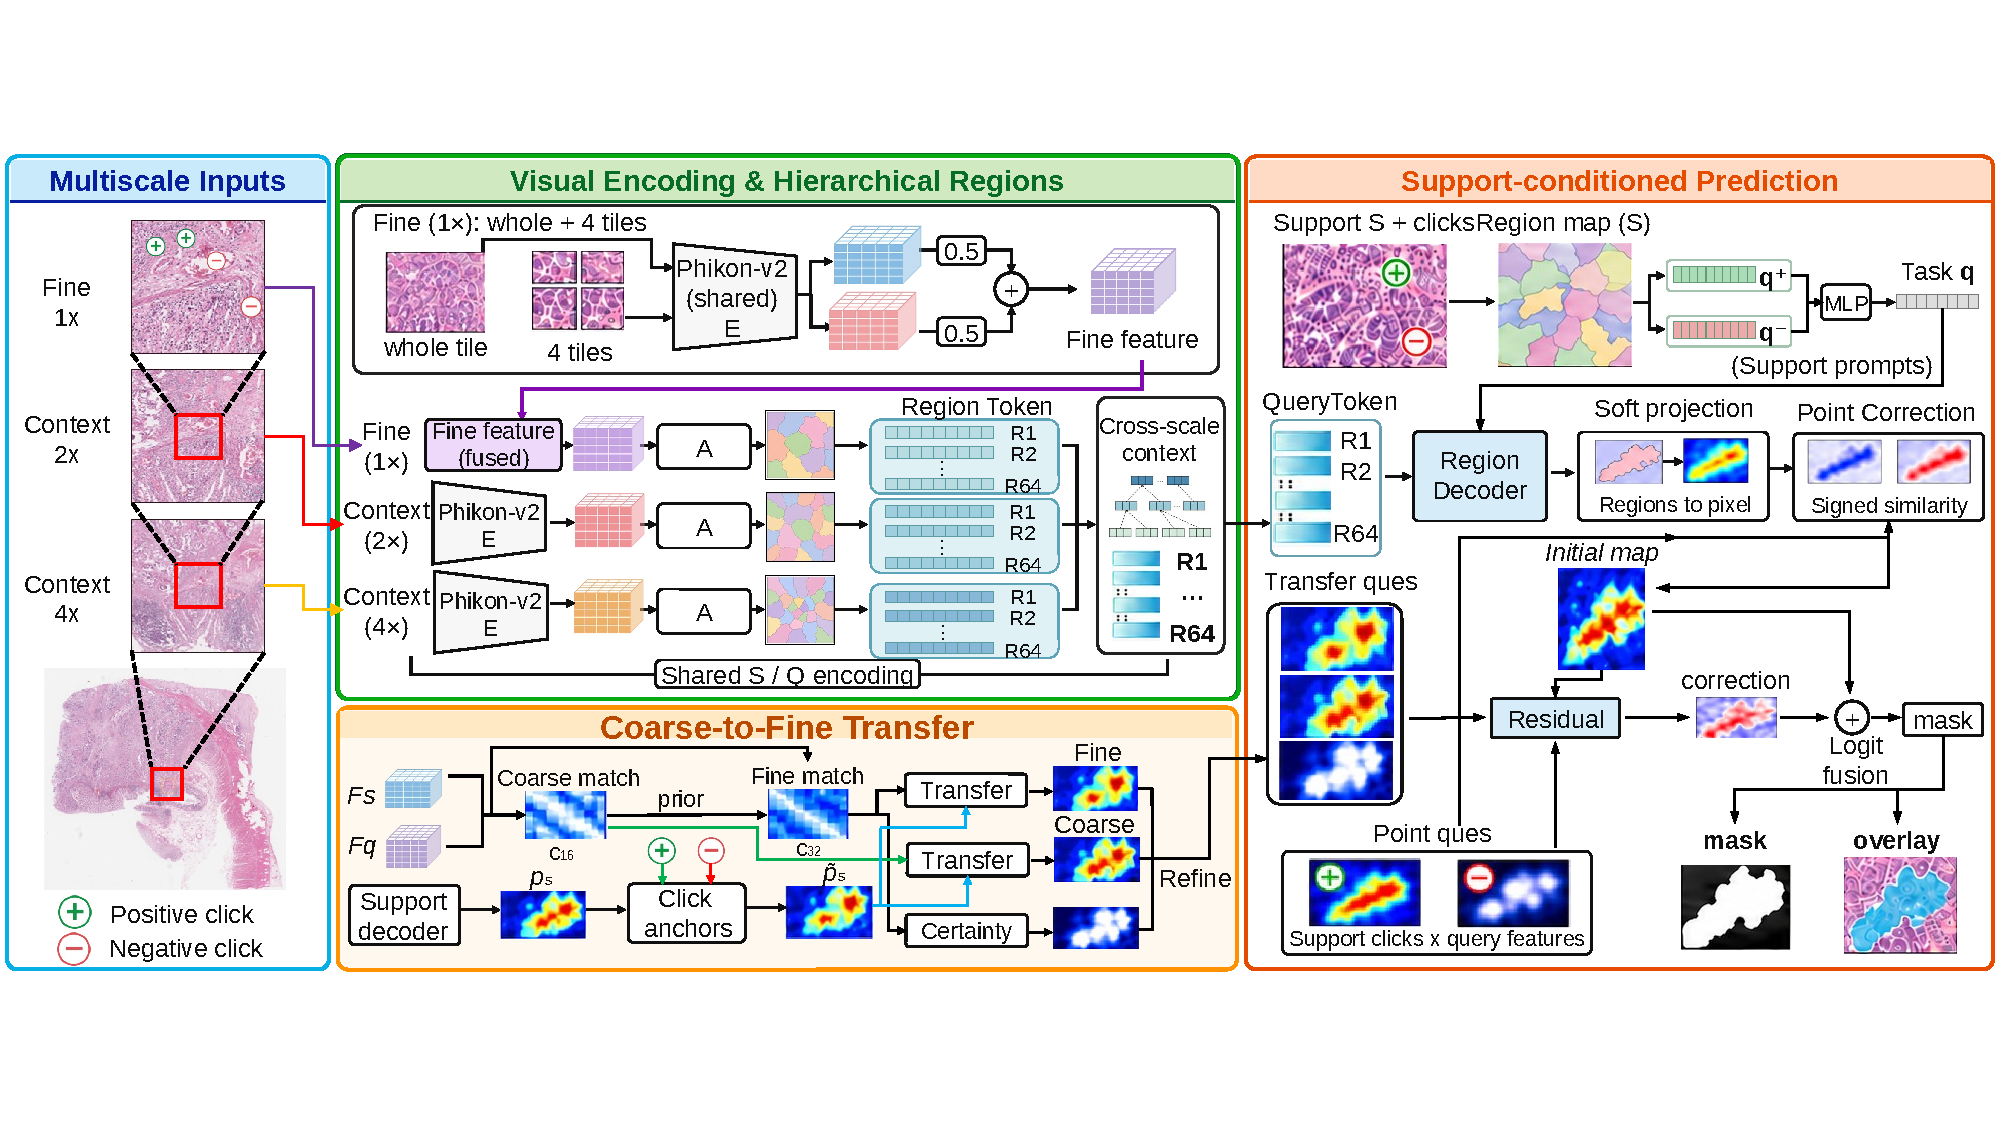
\includegraphics[width=\textwidth,trim=0 72bp 0 72bp,clip]{figures/method.pdf}
\caption{FewClick同片支持—查询分割框架。共享且冻结的Phikon-v2特征结合$1\times$、$2\times$和$4\times$视野，并对整块与分块精细特征取平均。软分配$A$池化区域token，用于跨尺度上下文交互。正负支持点击生成提示汇总向量$q^+/q^-$和任务向量$q$，用于查询区域解码。软投影与正负点相似度修正得到$p_0$。相同路径预测支持概率，并在迁移前通过点击进行锚定。投影特征$F_S/F_Q$构成粗尺度及先验引导的细尺度对应$C_{16}/C_{32}$；下标表示网格尺寸。迁移概率、基于熵的确定性、初始预测及点线索共同输入有界残差头。上采样后的修正量加至初始\emph{logits}，随后通过sigmoid并以$0.5$为阈值生成掩码。远端查询不接收人工点击。组织示例与中间特征图仅作示意。}
\label{fig:overview}
\end{figure*}
FewClick通过正负支持条件建模与密集概率迁移，将点击定义的组织目标传播至同一切片的各区域，并利用多尺度区域上下文组织空间证据（图~\ref{fig:overview}）。

\subsection{由提示定义的组织分割}
每次交互定义一个目标与其余组织之间的二分类任务。设$W$为一张WSI，$S$为支持图像块，$\mathcal P^+$和$\mathcal P^-$分别为其正负点击集合，$Q$为查询图像块。模型预测为
\begin{equation}
 p_Q=f_\theta(Q\mid S,\mathcal P^+,\mathcal P^-).
\end{equation}
支持图像块与远端查询图像块位于同一切片的不同物理位置。远端图像块评价要求二者的最大输入覆盖范围互不相交。更换切片或目标时，使用新的支持示例。训练使用支持与查询标注；推理仅使用二者的图像及支持点击。

\subsection{整块与分块特征融合}
\label{sec:fusion}
组织结构与精细构造需要不同的采样密度。对于每个支持或查询位置，我们提取同心的精细视野以及$2\times$、$4\times$物理视野，并将其分别缩放至$512\times512$。所有视野共享一个冻结的公开Phikon-v2骨干网络。

精细视野包含两条编码路径。一条编码完整图像块；另一条将其划分为四个互不重叠的$256\times256$分块，将各分块缩放至$512\times512$，并编码为原生$32\times32$空间token。将四个网格拼接后，在$64\times64$分辨率上恢复其空间排列。我们将整块网格对齐至这一分辨率，并融合两种表征：
\begin{equation}
 E_f=\tfrac12\operatorname{Align}(F_{\rm whole})
     +\tfrac12\operatorname{Stitch}(F_1,F_2,F_3,F_4).
\label{eq:fusion}
\end{equation}
更大的视野提供区域上下文。每个位置需要七次骨干网络编码：一次完整精细图像块编码、四次分块编码和两次上下文视野编码。

\subsection{提示条件下的区域层级}
\label{sec:regions}
\paragraph{空间上下文池化。}
每个视野在$64\times64$特征网格上构建$64$个$256$维区域token。令$F_s(x)$表示尺度$s\in\{f,m,c\}$上的投影特征，$a_s(x,k)$表示分配头的输出。区域$k$在规则$8\times8$网格上具有锚点$c_k$。位置$u(x)$与锚点$c_k$均位于$[-1,1]^2$，其软分配和池化token为
\begin{align}
 A_s(x,k)&=\operatorname{softmax}_{k}\!\left(a_s(x,k)-\frac{\|u(x)-c_k\|^2}{0.08}\right),\label{eq:assignment}\\
 r_{s,k}&=\frac{\sum_x A_s(x,k)F_s(x)}{\max(\sum_x A_s(x,k),10^{-6})}.
\end{align}
分配头以零初始化，并由分割监督更新。共享融合映射利用图像特征处理这些token；辅助细胞上下文与计数输入均固定为零。分配正则项对各视野的分配总量均衡、熵与紧致性项取平均，其权重分别为$0.01$、$0.001$和$0.01$。

\paragraph{跨尺度上下文。}
相邻尺度间的连接由物理重叠关系定义。我们将子视野映射至父视野的中央区域，累计二者分配图之间的重叠乘积，并为每个子区域保留至多四个有效父区域。此离散建边过程不参与计算图求导。稀疏的自底向上注意力依次更新中间尺度和粗尺度token。精细尺度token接收来自父区域及祖先区域的自顶向下注意力残差，并由一个零初始化可学习标量的双曲正切值进行门控。区域中心和面积均在共同的$4\times$坐标系中表示。

\paragraph{正负提示编码。}
我们在每个支持点击处对精细尺度分配图进行插值，并池化对应的区域token。集合编码时，归一化token结合位置、正负符号及可学习尺度嵌入，其中尺度索引固定。点击坐标位于$[0,1]^2$。共享的两层、四头集合编码器~\cite{lee2019settransformer}和可学习查询池化分别将正负集合汇总为$q^+$与$q^-$。二者的对比关系定义任务token：
\begin{equation}
 q=\operatorname{MLP}([q^+,q^-,q^+-q^-]).
\end{equation}

\paragraph{区域解码与像素投影。}
$192$个区域节点接收尺度嵌入。查询节点对带有位置和正负符号嵌入的支持提示token执行交叉注意力，并融合任务、几何及正负余弦相似度信息。图解码器保留包含自连接的尺度内六近邻连接与相邻尺度间的双向边。二分类头预测精细区域logits $o_k$。经上采样和归一化的分配将区域概率投影至像素：
\begin{equation}
 p_r(x)=\sum_k\bar A_f(x,k)\,\sigma(o_k).
\label{eq:projection}
\end{equation}
我们将该概率截断至$[10^{-6},1-10^{-6}]$，再转换为像素logits。相同的支持条件路径也用于预测支持掩码。

\subsection{正负点相似度修正}
\label{sec:point}
区域编码上下文，而点击位置提供直接的外观示例。共享$1\times1$投影将精细支持与查询特征从$256$维映射至$64$维。我们在点击处采样支持特征，并计算它们与归一化查询特征之间的余弦相似度。

正负点击各自的最大与平均相似度、正负最大相似度之差、缩放至$64\times64$的区域概率$p_r$及其不确定性$4p_r(1-p_r)$组成七个输入通道。卷积头预测修正量，经上采样后加至区域预测得到的logits。其最后一层以零初始化。此路径同时生成初始查询概率$p_0$与支持概率$p_S$。

\subsection{由粗到细的密集概率迁移}
\label{sec:transfer}
我们通过密集支持—查询对应关系迁移预测的支持概率场。

\paragraph{由点击锚定的支持概率。}
令$\bar p_S=\operatorname{Resize}_{32}(\operatorname{stopgrad}(p_S))$。正负点击场$g^+$与$g^-$分别累加同符号点击处的单位峰值高斯函数，其在$[0,1]^2$坐标中的标准差为$1/32$。锚定后的概率为
\begin{equation}
 \widetilde p_S=\frac{\bar p_S+4g^+}{1+4g^++4g^-}.
\label{eq:anchor}
\end{equation}
这会在点击附近约束待迁移的支持证据。

\paragraph{由粗到细的对应关系。}
平均池化将投影后的$64\times64$特征转换为$32\times32$和$16\times16$网格。特征归一化后，查询—支持余弦相似度形成矩阵$K_{32}$与$K_{16}$。以温度$\tau=0.1$沿支持位置进行softmax，得到粗尺度对应$C_{16}$。扩展$\mathcal U$将每个粗尺度查询行复制至四个子位置，并将每个支持位置的概率质量均分给四个子位置。令$\Pi_{32}=\max(\mathcal U(C_{16}),10^{-8})$，则有
\begin{align}
 C_{16}&=\operatorname{softmax}_{S}(K_{16}/\tau),\\
 C_{32}&=\operatorname{softmax}_{S}\!\left(K_{32}/\tau
                  +0.5\log \Pi_{32}\right).
\label{eq:correspondence}
\end{align}
矩阵的行与列分别索引查询和支持位置；$C_{16}$与$C_{32}$的尺寸分别为$256\times256$与$1024\times1024$。

\paragraph{迁移与残差细化。}
将概率网格展平为向量后，对应关系迁移锚定后的概率场（$\operatorname{Pool}$为$2\times2$平均池化）：
\begin{equation}
 t_{32}=C_{32}\widetilde p_S,\qquad
 t_{16}=C_{16}\operatorname{Pool}(\widetilde p_S).
\end{equation}
迁移后的向量恢复为空间网格。匹配确定性为一减去$C_{32}$各行的熵与$\log 1024$之比。精细迁移、缩放后的粗尺度迁移、确定性、$p_0$、$4p_0(1-p_0)$、正负最大相似度及其差值在$32\times32$网格上组成八通道输入$z_Q$。一个$3\times3$卷积、GELU及一个$1\times1$卷积预测有界logit残差：
\begin{equation}
 p_Q=\sigma\!\left(\operatorname{logit}(p_0)
                +\operatorname{Up}[2\tanh h(z_Q)]\right).
\label{eq:residual}
\end{equation}
上采样将输出恢复至$512\times512$分辨率。密集迁移用于远端任务；本图交互使用区域和点修正路径。完整模型保留点击锚定与粗尺度先验。

\subsection{训练目标与优化}
\label{sec:training}
训练涵盖本图交互、同片目标存在迁移与目标缺失迁移。固定队列包含$9{,}500$个任务：$4{,}000$个本图任务、$5{,}000$个远端目标存在任务和$500$个远端目标缺失任务。每次更新累计四个任务，共进行$2{,}375$次更新。目标函数为
\begin{equation}
 \mathcal L=\mathcal L_Q+0.25\,\mathbf{1}_{\rm remote}\mathcal L_S
                  +0.1\mathcal L_{\rm click}+\mathcal L_{\rm assign}.
\end{equation}
分割损失结合有效像素上的二元交叉熵、用于目标存在任务的soft Dice，以及权重为$0.5$的边界带交叉熵。对于目标缺失查询，使用平均预测概率的$0.1$倍替代Dice项。当正负标签均存在时，交叉熵对正负像素损失等权平均。点击损失约束正负提示处的支持预测。远端任务的$\mathcal L_{\rm assign}$对支持和查询图像取平均。

我们使用AdamW，学习率与权重衰减均为$10^{-4}$。公开骨干网络保持冻结，下游模块重新初始化。功能检查使用训练数据，正式训练前再次重新初始化下游模块。推理使用最后一次更新后的模型，并固定概率阈值为$0.5$。

\subsection{基于单个支持集的整片推理}
\label{sec:wsi}
每个“切片—目标”组合使用一个支持图像块及其正负点击。查询窗口复用该支持状态；更换切片或目标时重新设置。设支持精细视野尺寸为$(b_w,b_h)$，查询网格使用$\lfloor b_w/2\rfloor$与$\lfloor b_h/2\rfloor$的步长。通过与边缘对齐的窗口补全最后一行和最后一列，并将支持位置纳入网格。上下文视野保持同心，图像外部使用白色填充。

每个窗口的概率通过像素中心对齐的双线性插值映射至标注网格。在重叠位置，对所有覆盖窗口取平均：
\begin{equation}
 p_W(x)=\frac{\sum_j\mathbf{1}[x\in\Omega_j]p_j(x)}
                   {\sum_j\mathbf{1}[x\in\Omega_j]},\qquad
 M_W(x)=\mathbf{1}[p_W(x)\geq0.5].
\end{equation}
每个输出像素必须至少获得一次预测贡献。整片Dice对每个有效标注像素仅计数一次。严格远端评价移除所有受影响窗口的精细输出矩形之并集；受影响窗口指其$4\times$输入覆盖范围与支持区域的$4\times$输入覆盖范围相交的窗口。在读取标注进行评分之前，预测已固定；未标注像素不参与评价。
